\subsubsection{Entropy}

You may recall from high school physics that entropy has something to do with thermodynamics.  Why in the world is it used to describe passwords?  

Claude Shannon coined the use of the term “entropy” in information theory when he recognized the formula he had developed for measuring information also occurred in statistical mechanics, where it was called entropy!  He used the letter H to represent it since it was so in Boltzmann’s famous H theorem, which has to do with molecules moving to equilibrium.
\begin{figure}[h]
\centering
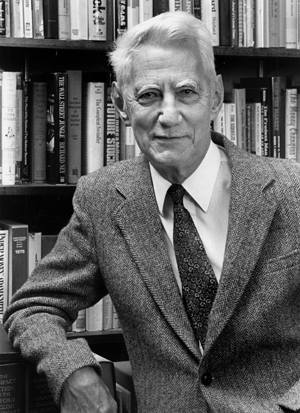
\includegraphics[height=3cm]{Claude_Shannon.jpeg}
\caption{Claude Shannon}
\end{figure}

For passwords “Entropy” denotes the uncertainty in the value of a password. 

Entropy of passwords is conventionally expressed in bits, which brings you back to high school math.  That’s right logarithms!  If your alphabet consists of 26 letters, say and you require 8 letters in your password then there are \(26^8\) possible passwords. That can be expressed as entropy with

\[H = \log_2(26^8) = 37.6 bits\]

More information is provided by NIST at \url{https://nvlpubs.nist.gov/nistpubs/SpecialPublications/NIST.SP.800-63-2.pdf}.

Humans don’t do random very well, so in reality, much of the possible space is never taken by self-selected passwords, so in practice the entropy is overstates the value.

Of course, modern computers with access to the password hash file can make quick work of this.  So finding ways to prevent or throttle password guessing is important!  Or, better yet, don’t rely entirely on passwords!
